\section{Wprowadzenie}
	\begin{frame}{Wprowadzenie}
	\begin{itemize}
	    \item 	wywodzą się z praktyki inżynierskiej
	    \item  do kreślenia elementów konstrukcyjnych w przemyśle  używano elastycznej listewki drewnianej (liniału) nazywanej giętką (ang.spline)
	    \item liniał prowadzono przez zadane punkty za pomocą  ciężarków
	    \item liniał uginał się wzdłuż krzywej „najgładszej”
	    \item  alternatywa: użycie krzywików
	   \end{itemize}
	   \begin{figure}
	       \centering
	       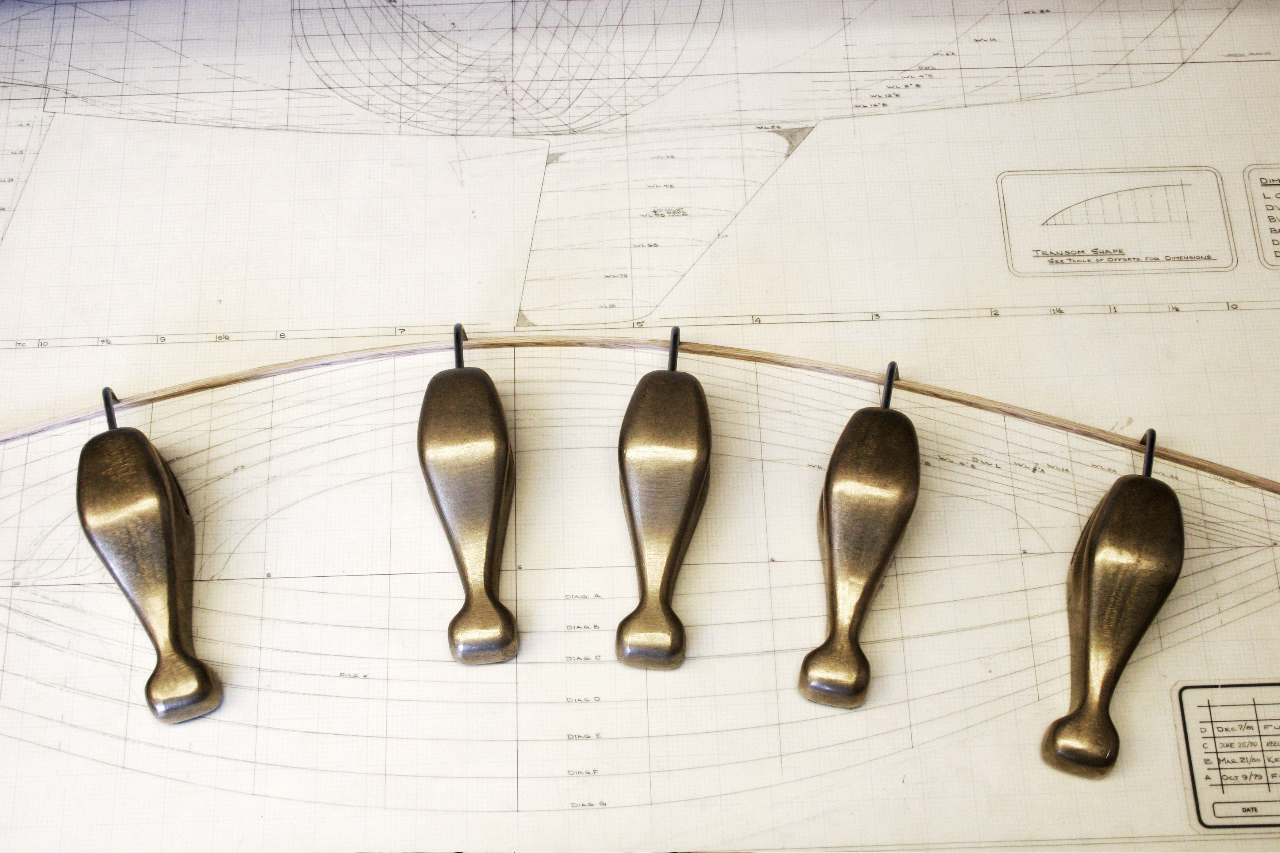
\includegraphics[width=4cm]{img/4/spline_figure.jpg}
	       \caption{źródło: http://www.alatown.com/spline/}
	       \label{fig:my_label}
	   \end{figure}
        
     %   $s(x)$ - funkcja $\newline$
     %   $s''(x)$ - krzywizna, dx - długość łuku $\newline$
     %   $s,\ s',\ s'' $ - ciągłe w $[x_{i},x_{n}] \newline$
     %   local curvature: $\frac{f''(x)}{(1+f'(x))^{\frac{5}{2}}}$
     %  \[
     %   	\min ! \int_{x_{i}}^{x_{n}}\underbrace{[s''(x)]^{2}dx}_{E_{p}}
      %      \Rightarrow w_{3}(x)
      %      \ \ \textrm{na} \ \ [x_{i},x_{i+1}]
      %  \]
      % \[
      %  	\textrm{"strain energy"} = \int_{a}^{b} 
      %      \frac{(f''(x))^{2}}{(1+f'(x))^{\frac{3}{2}}}dx
      %  \]
        
	\end{frame}
    %%%%%%%%%%%%%%%%%%%%%%%%%%%%%%%%%%%%%%%%%%%%%%%%%%
    \begin{frame}{Definicja funkcji sklejanej}
    	\begin{exampleblock}{}
    		Funkcję $s(x) = s(x, \Delta n)$ określoną na $[a,b]$ nazywamy funkcją sklejaną stopnia m $(m\geq1)$ jeżeli:
            \begin{itemize}
            \item $s(x)$ jest wielomianem stopnia $ \leq m$ na każdym $[x_{i},x_{i+1}]$
            \item $s(x) \in C^{m-1}[a,b] $
            \end{itemize}
            $\newline$
            $\Delta n$ - podział $[a,b]$ na (n-1) podprzedziałów przez węzły: 
            $a=x_{1}<x_{2}<...<x_{i}<...<x_{n}=b$
    	\end{exampleblock}
	
    \end{frame}
    \begin{frame}
    
		\begin{figure}[h]
			\includegraphics[width=.9\linewidth]{img/4/spline_img_4}
		\end{figure}
    \end{frame}